\documentclass[letterpaper, 10pt, draftclsnofoot, compsoc, onecolumn]{IEEEtran}
\usepackage{graphicx}
\usepackage{textcomp}
\usepackage{comment}
\usepackage{hyperref}
%\usepackage{digsig} %not a default package... just for signature field on final page.
\usepackage{url}
\graphicspath{ {} }
\hypersetup{pdftex, colorlinks=true, linkcolor=black, citecolor=blue, filecolor=blue, urlcolor=blue, pdftitle=SYSTEMS AND SOFTWARE REQUIREMENTS SPECIFICATION (SSRS) TEMPLATE, pdfauthor=Clinton Jeffery, pdfsubject=, pdfkeywords=}

% Page layout (geometry)
\setlength\voffset{-1in}
\setlength\hoffset{-1in}
\setlength\topmargin{0.5in}
\setlength\oddsidemargin{.75in}
\setlength\evensidemargin{.75in}
\setlength\textheight{8.278in}
\setlength\textwidth{6.5in}
\setlength\footskip{0.561in}
\setlength\headheight{0.5in}
\setlength\headsep{0.461in}

\begin{document}
\pagenumbering{gobble}
\title{Winter Progress Report - Forge Explorer}
\author{Griffin Gonsalves}
\maketitle
\hspace*{\fill}\IEEEauthorblockA{CS462 Capstone - Winter 2017}\hspace*{\fill}
\vspace{8cm}


\begin{abstract}
This document expands upon Group 20's progress with the Forge VR Explorer, a collaborative model viewing app, as it stands through week 10 of development. This document focuses on my impressions, results, and findings for the term. The document also includes a project summary, details of project related problems with changes and solutions, as well as a week-by-week breakdown of the progress of development. 
\end{abstract}
\IEEEpeerreviewmaketitle

\newpage 

\setcounter{tocdepth}{2}
\renewcommand\contentsname{}
\tableofcontents

\bigskip
\clearpage
\pagenumbering{arabic}

\section{Project Recap}
%Purposes and Goals

Our team's project seeks to improve and build upon the vrok.it hackathon project, increasing the usability while simultaneously integrating more features using Forge API's. The Forge API collection has a number of API's that facilitate development with 3D modeling and creating applications like ours. The end product will be capable of uploading CAD files via local user files or through Data Management’s A360, displaying the files as models through the File Viewer, file conversion with the Model Derivative, viewing the site on a mobile device via QR scanner and then viewing the site, specifically models, in stereoscopic VR with Google Cardboard.

\section{Current Progress}
Following our winter midterm progress report I worked towards updating the site more regularly, and made some commits changing the site content and placement of key items, such as the Forge Viewer, and the sizing of the split html page. In doing this I discovered the site was a little more resistant to my changes than I was hoping, but because the other changes were working fine, I decided to move on. The next task I turned my focus to was sorting out the keyboard and mouse controls for the viewer, since we want to have a demo that allows for conventional controls. After doing some research on the Autodesk developer portal(https://developer.autodesk.com/) I found that I could adjust our instance of the Forge Viewer with a Javascript extension, or by modifying one that was already being used. I decided to investigate further and see what I could do with what was already in the files, as recommended by our project leaders. I ended up enabling the first-person functionality by adjusting several constraints within the javascript file for the viewer.

\begin{figure}[h]
	\centering
	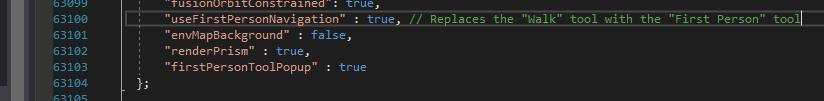
\includegraphics[scale=.5]{firstperson1.jpg}
	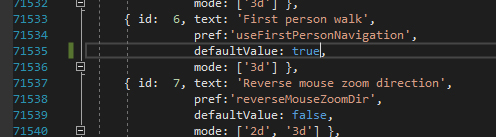
\includegraphics[scale=.5]{firstperson2.jpg}
\end{figure}


\section{Remaining Tasks}
The thing I would like to focus on, as well as our team, is to find out what makes a better UI in terms of a Web program like ours. I have made efforts to adjust what the site looks like, but haven't felt like there is a sizable difference in terms of its overall friendliness and usability besides the first person and keyboard controls and the other API's we have included. With what time I have left I want to clean up the project files, and implement a final version of the page to update to for our demo. I will likely spend considerable time over spring break or at the beginning of Spring term to pursue these additional changes in light of my struggles with development over the course of the term and considering the overall goals of the project.


\begin{comment}
\section{Retrospective}

\begin{center}
\begin{tabular}{ |p{0.3\linewidth}|p{0.3\linewidth}|p{0.3\linewidth}| } 
 \hline
 \textbf{Positives} & Deltas & Actions \\ 
\hline
After Autodesk University was over our client has become much more available to answer our questions and concerns regarding the project & Planning for future events with the team and making sure there aren't any major conflicts. & The team will communicate questions through emails, and scheduling conflicts will be resolved during client meetings. \\
\hline
  & Better team communication. & This could be accomplished by setting up an in person weekly meeting that happens at the same time every week. \\
\hline 
  & Addressing problems or concerns regrading assignments or documentation. & If everyone in the group is having the same problem and we are not able to come up with a solution we need to ask our TA our one of the professors if they have the answer to the problem we are having. \\ 
 \hline
\end{tabular}
\end{center}
\end{comment}

\section{Weekly summaries}

\subsection{Winter Week 1}
 Following our initial plan for updating the design, I began with opening up the project files to understand more of the backend, and how each project file was related to each other. I have designed and implemented a few different web sites before, but I hadn't worked on a server-based node.js project like this.  I began implementing the site through GitHub hosting, and the initial page began to load after my first week of work on the site. As it turned out, I was not necessarily prepared for all of the learning of the tools that were suddenly thrust upon me. However, we soon discovered that GitHub hosting was inadequate for our project as the node resources require a server interface. I was very unfamiliar with the node tools, and Heroku page setup as they are both robust and powerful applications, but learned enough to assist move the project off of the GitHub Pages site. I was a bit bummed that the initial plan didn't work out as we had hoped, but I think the result is perfectly fine-the site has not had any major hosting issues since the transition.

\subsection{Winter Week 2}

 During week 2 of our development phase, we made a transition to Heroku for our hosting service. This change delayed us slightly, but overall is for the better since we now have a server to push our project files to. During this week we reached out to our project sponsor at Autodesk, Patti Vrobel, to assist us in this setup. We also began planning our transition to our next phase of development on our schedule. Each of us spent time learning Git essentials for our machines, and set up so we could each push updates to the server. I have begun doing more investigation with project files and how we will navigate with multiple viewers active at once. Once we are able to test out key functions of the site I plan on beginning to update the site layout next week.
\subsection{Winter Week 3}

Another week down, and things have begun to pick up more speed. We were able to meet again with our client and Kean Walmsley from Autodesk via conference call, and got heaps of useful information on the site and some guidance for our development. After setting up our upload pipeline for Heroku, I started planning out what some of the layout changes could be and what I wanted the site to end up looking like. I spent some time brushing up on node.js, and some of its useful features. At the beginning of next week I hope to begin pushing some changes to the site so that the layout will be adjusted and some other site features can be added later down the line. Additionally, we hope to have an updated development schedule early in the week.
\subsection{Winter Week 4}

Overall, this week was not quite as smooth as we had hoped, but still progress is being made nonetheless. Spending more time with the project, I discovered that the main landing page is actually a compilation of pages being loaded at once, making the adjustment of the layout more complex than I had originally thought. I suspect this has to do with node running a live session and pages loading in asynchronously. I have the removal and updating of several pages for the project site near-ready, however, I had to wait until Paul and Shawn were completing their portions of the project. I hope to push these updates next week and start working with the team and Autodesk on A360 integration and possibly on the movement within the Autodesk Viewer. Hopefully this week we'll be able to do some testing with our Google Cardboard as well with the new models, and various model types early this week so we can develop a more optimal setup for the Viewer on our page. Overall, I think the website will look great once the authentication changes have been completed.
\subsection{Winter Week 5}

This week I was a bit bogged down in other classwork, but I was still able to contribute to our project and help the team. I'm very glad that Paul and Shawn were able to make significant progress on the authentication for the site, and now we shouldn't have any other significant setbacks moving forward. During this week, I developed a new prototype for the website layout, now that we have updated our design with our current technology and have tested our authentication properly. It is exciting to see the project come together so suddenly, and that we are all getting more ideas while we are developing. I hope in the next week after we complete our necessary progress report documentation that we will be able to get creative and put some awesome work into the project for the rest of development. In order to do this, we plan on meeting again with our friends at Autodesk via phone call or Skype during week 6 and 7 in order to address any pressing questions we may have with APIs or our project in general.

\subsection{Winter Week 6}
This week was spent primarily focusing on preparing the application for an "alpha" state. We encountered some problems while fixing some portions of our implementation of the authentication portion which pushed some of our recording and general planning of our progress report later in the week, but we managed to get everything done on time. I did take the revisions to our documents seriously, and revised some of my sections in each document as well. Next week I will be implementing more UI changes, and hopefully will have more questions to ask the Autodesk team, that way I can learn as much as possible in these coming weeks. I hope the Forge Viewer also gets updated soon as well, that way the stereoscopic view will look even better for our Google Cardboard demo when we get to it. Looking forward to this week!
\subsection{Winter Week 7}
This week I made an effort to push some more changes to the website, and made some headway to including keyboard controls enabled by default in the Forge Viewer. This would be a good step toward one of our core goals- improving the usability of the project. I began by editing the existing Forge Viewer javascript extension that is in use on the site, but now I am thinking that perhaps the best option might be to create our own extension for the Viewer, since that would allow us to try out more of our own changes should we choose to add more to the project. In any case, the updated Viewer has the option to explore the model in first person using the standard WASD keyboard layout(as desired). Ideally, I will be able to work the functionality in this week with help from the Autodesk team, and my group that way we can focus on other parts of the project since the Authentication implementation is functioning as intended. It has been very busy the past few weeks, but hopefully the project continues to come together nicely.
\subsection{Winter Week 8}
During this week, I focused myself on trying to get some more UI changes pushed to the main site, along with some more work towards the addition of keyboard controls. I tried to follow along with Kean Walmsley's blog on Javascript extensions for the Forge Viewer to assistance and guidance. My current plan is to modify one of the existing extensions to minimize the overhead so I can continue on the interface. I hope this week me and the rest of the group can meet up and use teamwork to move our project into the beta stage. Hopefully by the end of the week I will have completed my modifications to the extension, which will put our progress further ahead.


\section{Team Evaluation}

Overall, I'd say our team has been operating pretty normally this term. I feel that there was still some slight angst going into the term from the start, which could have been caused by previous events. During Fall term Paul and myself had tried to settle a conflict regarding contributions last term. I felt as though we had settled everything before the end of Fall term, so I thought it was a bit strange communication was sparse and nobody seemed to want to jump on our development. I suppose this all could be normal after all, but I didn't exactly sense a positive communication environment. I still decided to continue with the plan and started on porting the project to our github pages site. As mentioned before we needed to switch to a Node.js supported framework, so Shawn and Paul assisted in working on an alternative. In the coming weeks, Paul and Shawn worked hard to finish porting the updated API information to the updated server file. During this time, I was focusing on other classwork and midterms. It was during this time I began to struggle significantly and my communication suffered as a result. At the end of week 8, I returned home to California to visit with family and take care of some other personal concerns.  During this time, I failed to recognize that I should have reached out to someone(Kirsten, Shivani) about what was going on which caused some concern. When I returned, I was able to visit with Kirsten and talk about the term. 

For me, a considerable amount of time had to be spent catching up on other classwork as I returned back again in Corvallis. However, I was feeling that I was in a much better state, and was able to resume communication with my team and pushed forward on our development. As a whole, I'd say Shawn has done a great job staying consistently on top of everything for the project, and has been a good leader. Paul, who I mentioned earlier, has done a lot of work on the technical end of the project, especially where me and Shawn were having difficulty. For myself, I feel that I have functioned best as the team's designer, helping with planning and ideas but had difficulty communicating when I needed help or assistance in tackling objectives. Overall, I'd say we each have contributed equally in different areas, and function well as a development team. Of course, I'd love for our group to have closer and more thorough  communication during development which is something I feel the team could have benefited from. 
\end{document}
